%########################################
%CS 461 CAPSTONE 
%GROUP 20 - Griffin Gonsalves, Paul Kwak, Shawn Cross
%FALL 2016
%########################################
\documentclass[letterpaper, 10pt, draftclsnofoot, compsoc, onecolumn]{IEEEtran}
\usepackage[latin1]{inputenc}
\usepackage[T1]{fontenc}
\usepackage[english]{babel}
\usepackage{amsmath}
\usepackage{amssymb,amsfonts,textcomp}
\usepackage{color}
\usepackage{array}
\usepackage{supertabular}
\usepackage{hhline}
\usepackage{color,soul}
%\usepackage{biblatex}
\usepackage{cite}
\usepackage{hyperref}
%\usepackage{digsig} %not a default package... just for signature field on final page.
\usepackage{url}

\usepackage{comment}

\hypersetup{pdftex, colorlinks=true, linkcolor=black, citecolor=blue, filecolor=blue, urlcolor=blue, pdftitle=SYSTEMS AND SOFTWARE REQUIREMENTS SPECIFICATION (SSRS) TEMPLATE, pdfauthor=Clinton Jeffery, pdfsubject=, pdfkeywords=}
\usepackage[pdftex]{graphicx}
% Outline numbering
\setcounter{secnumdepth}{4}
\renewcommand\thesection{\arabic{section}}
\renewcommand\thesubsection{\arabic{section}.\arabic{subsection}}
\renewcommand\thesubsubsection{\arabic{section}.\arabic{subsection}.\arabic{subsubsection}}
\renewcommand\theparagraph{\arabic{section}.\arabic{subsection}.\arabic{subsubsection}.\arabic{paragraph}}

\parindent0pt
\parskip 1.5ex plus 0.2ex minus 0.1ex
\makeatletter

\def\subsubsection{\@startsection{subsubsection}% name
                                 {3}% level
                                 {\z@}% indent (formerly \parindent)
                                 {1ex plus 0.1ex minus 0.1ex}% before skip
                                 {1ex}% after skip
                                 {\normalfont\normalsize}}% style

\newcommand\arraybslash{\let\\\@arraycr}
\makeatother
% Page layout (geometry)
\setlength\voffset{-1in}
\setlength\hoffset{-1in}
\setlength\topmargin{0.5in}
\setlength\oddsidemargin{.75in}
\setlength\evensidemargin{.75in}
\setlength\textheight{8.278in}
\setlength\textwidth{6.5in}
\setlength\footskip{0.561in}
\setlength\headheight{0.5in}
\setlength\headsep{0.461in}
% Footnote rule
\setlength{\skip\footins}{0.0469in}
\renewcommand\footnoterule{\vspace*{-0.0071in}\setlength\leftskip{0pt}\setlength\rightskip{0pt plus 1fil}\noindent\textcolor{black}{\rule{0.25\columnwidth}{0.0071in}}\vspace*{0.0398in}}
% Pages styles
\makeatletter
\newcommand\ps@Standard{
  \renewcommand\@oddhead{\hfill }
  \renewcommand\@evenhead{\@oddhead}
  \renewcommand\@oddfoot{\foreignlanguage{english}{\textcolor{black}{SSRS Page }}\foreignlanguage{english}{\textcolor{black}{\thepage{}}}}
  \renewcommand\@evenfoot{\@oddfoot}
  \renewcommand\thepage{\arabic{page}}
}
\newcommand\ps@FirstPage{
  \renewcommand\@oddhead{}
  \renewcommand\@evenhead{\@oddhead}
  \renewcommand\@oddfoot{}
  \renewcommand\@evenfoot{\@oddfoot}
  \renewcommand\thepage{\arabic{page}}
}
\makeatother
\pagestyle{Standard}
%\setlength\tabcolsep{1mm}
\renewcommand\arraystretch{1.3}
% footnotes configuration
\makeatletter
\renewcommand\thefootnote{\arabic{footnote}}
\makeatother
\title{Forge VR Explorer Requirements}
\author{Shawn Cross, Griffin Gonsalves, Paul Kwak}
\date{2016-11-3}


\begin{document}

\clearpage\setcounter{page}{1}\pagestyle{Standard}
\thispagestyle{FirstPage}

\bigskip

{\centering\selectlanguage{english}\bfseries\color{black}
Forge VR Explorer Design Document
\par}

\bigskip

{\centering\selectlanguage{english}\bfseries\color{black}
December 2 2016
\par}
\bigskip
\bigskip
\bigskip
\bigskip
\bigskip
\bigskip
\bigskip
\bigskip
\bigskip
\bigskip
\bigskip
\bigskip
%\begin{center}
%	
\includegraphics[scale=0.8]{forge_logo.png}
%\end{center}

\vfill
{\centering\selectlanguage{english}\bfseries\color{black}
Abstract
\par}

{\centering\selectlanguage{english}\mdseries\color{black}
	The Forge VR Explorer branches from an Autodesk prototype project called Vrok-It, which is a simple web-based 3D 
	model viewer and mobile virtual reality (VR) explorer. The project will expand upon its ability to display uploaded 3D 
	models in browser and in VR, and improve its accessibility. Conventionally, viewing 3D models in VR is a challenge if 
	you have model files on many devices, or have a headset that only works in conjunction with a smart-phone. The 
	Forge VR Explorer aims to do this by utilizing a web-based software that uses the features of the Autodesk Forge API. 
	The project will also be expanded with new ideas and stretch goals as the project is developed.
\par}
\clearpage
{\centering\selectlanguage{english}\bfseries\color{black}
TABLE OF CONTENTS
\par}

\bigskip

\setcounter{tocdepth}{2}
\renewcommand\contentsname{}
\tableofcontents

\bigskip
\clearpage

\section{Introduction}
The software implemented is a web application capable of accomplishing several tasks. The software allows for the upload of CAD files, renders them on the website using the various Forge APIs, allows the transfer and rendering of the models onto a user's mobile device, and then has the capability to allow the user to view the models using Google Cardboard or similar VR headsets. This document aims to delve into the design of each piece of functionality and seeks to expand its design and structure.
\subsection{Scope}
The scope of this document covers the information regarding user experience data flows, the software design description and the design structure of the software. This design document includes information critical to the development of the project as a whole. This document does not cover specific implementation decisions or quality requirements.
\subsection{Purpose}
The purpose of this software design document is to describe the user experience flows and provide the software design description to its intended audience. Additionally, this document provides a framework for the project that the developers will be using in order to assess the progression of the software through its development lifespan. This includes the detailed description of critical design entities, components, and systems working together in the project.
\subsection{Intended audience}
This document is targeted at developers building and implementing the software, and the stakeholders who include: Patti Vrobel, the Autodesk Forge API team,  and developers of the original "Vrok-it" project that this is based off of. Core stakeholders also are working with the project group in order to maximize the projects potential.

\subsection{Definitions}
\begin{description}
	\item{CAD} Computer Aided design is software used to design and view 3D models.

	\item{CAD file} The type of files that can be uploaded to the website for viewing in the Forge viewer. 
	We will  narrow down what types of files can be used as we progress through the development process.

	\item{FORGE}~\cite{forge2016} A collection of API services provided by Autodesk that provide 3D modeling services and tools.

	\item{Forge Viewer} This is one of the APIs in Forge. It displays 3D models from CAD files and also allows
	for user interaction.
	
	\item{Model Derivative API} This is another API in Forge. It can generate SVF files that we can utilize in the application from other model filetypes.
	
	\item{VR} Acronym for virtual reality, typically a peripheral device or smartphone

	\item{exploding model} A model viewing functionality that separates components from their original locations in order to gain an alternate view of the model.

	\item\textbf{SVF file} The file format used by the forge viewer
\end{description} 

\bibliography{bibfile}
\bibliographystyle{IEEETran}

\subsubsection{Influences on SDD preparation}
The SRS is the main influence on the SDD as it holds the requirements and features determined necessary by all the stakeholders. This drives the design to meet those requirements to properly satisfy all stakeholders. However, this also means that it sets the design constraints.

\subsubsection{Design verification and design role validation}
In order to verify that our software meets requirements, test cases will be used in order to walkthrough the system and demonstrate the actual funtionality of the software system. In terms of user experience the verification and validation will be mainly done through some primary tests with Autodesk with final okay coming from the clients.

\subsection{Design stakeholders and their concerns}
	The primary stakeholder for this project is Patti Vrobel who works for autodesk. User experience is a primary focus of both Patti and Autodesk, and serves as an overarching goal for the project. The project addresses this by adding and altering features to make the website more accessible for users.

\section{Design Views}

\subsection{Model Viewer}
\label{modelView}
The user must be able to see the model they uploaded from the cad file. This is accomplished by using the Forge Large Model Viewer, or Forge Viewer. The model must be able to be manipulated and explored with simple and intuitive controls. This includes both a viewer on a desktop machine as well as a separate viewer exclusively for the smartphone. Because this viewer is responsible for a large aspect of the project, ensuring the viewer is configured to run as smoothly as possible is essential.


\subsection{Interface Viewpoint: Interaction}
\begin{itemize}
	\item[]\textbf{Main Viewer Window} By default, there will be at least one viewer within the desktop website after a completed their file upload.  This includes the Viewer Controls component. The viewer uses a WebGL graphics backend that is integrated into the webpage, then called with the Forge API. If an error is detected, the viewer should fall back to an inactive state.
	
	\item[]\textbf{Viewer Controls} The viewer is interacted with by using the Large Model Viewer's API, which is a small set of controls in a compact interface that appears at the bottom of the viewer. This set of controls can rotate, zoom, explode, or toggle settings for viewing the model. If a keyboard is connected, then a set of keys can be used to control the viewer in a basic and straightforward manner.
	
	\item[]\textbf{Secondary Viewer}  The Main Viewer must control a separate instance of the Viewer that runs exclusively for the connected smartphone, and matches the exact position and viewing of the desktop viewer. The main viewer is also responsible for handling the controls for the second viewer. These viewers are hosted within the web page.
	

\end{itemize}
\subsection{Model Viewer Navigation}
This section of software includes an update to allow keyboard and mouse input as a new option for controlling the Forge Viewer. This is essentially what enables the model viewer to explore the model, and is a separate layer of control from the Viewer Controls. 
\subsection{Interface Viewpoint: Interaction}
\begin{itemize}
	\item[]\textbf{} 
	\item[]\textbf{} 
	\item[]\textbf{}  
	\item[]\textbf{}
	\item[]\textbf{} 
\end{itemize}
%placeholder
\begin{comment}


\subsection{Interface Viewpoint}
\begin{itemize}
	\item[]\textbf{} 
	\item[]\textbf{} 
	\item[]\textbf{}  
	\item[]\textbf{}
	\item[]\textbf{} 
\end{itemize}
\end{comment}


\subsection{Website Structure}
Because the website is the focus of the project, we are hosting a new version of the website utilizing a github project page for hosting. The requirements for the website are to properly host, arrange and display all of the components of the project. This includes the file uploading, authentication, the forge viewer, and mobile device connection software. The website must be simple to use, and appears intuitive for all users.

This addition is necessary in order to have control over the project hosting, and to test and deploy updates. Additional constraints to this view include limiting technical details of each component for the purpose of creating a prototype for the project's core user experience. 

\subsection{Interface Viewpoint: Structure}
\begin{itemize}
	 \item[]\textbf{Forge Viewer} Implementing the Forge Viewer into the page will involve calling the API from a script embedded in the page. The individual required files for the viewer are held in the site source files.
	
	\item[]\textbf{Forge Viewer Navigation} This component of the project encompasses the control modifications and adjustments made to the viewer to allow model exploring.
	 
	\item[]\textbf{File Upload} The file upload functionality will be available on the main page in a specific area.
	
	\item[]\textbf{Smartphone QR Code}  The smartphone QR code will also have its own page section and will be viewable on the main page of the site.
	
	\item[]\textbf{Model Derivative} This component is essential in preparing the model to be used in the viewer. It is used as a method of transforming a given model of one of many supported formats to SVG. This is accomplished by using an API call to the Model Derivative API.
	
	\item[]\textbf{Information and Other Site Content} The website will eventually come to encompass more content as the project progresses in development. These changes will be noted in blogs, and will be made visible on the project website. These additions to the site will most likely come as feature updates to previously described components or new features on new pages of the site.
\end{itemize}

\subsection{Local file upload}
	The user should be able to upload their own CAD files from a local storage device that they have access to. This will be some sort of button that is easily identifiable by the user that once selected will allow the user to browse through the local files on the current machine and select the CAD file that they would like to view. Once the file is selected the website should verify that the file is an allowed CAD drawing file. If the file is of the correct file type then the file should be converted to the SVF file type that is used by the forge viewer api. The user should be notified that the file was successfully uploaded to the website and the model that was in the file should be displayed in the list of choose-able models as well as displayed in the viewer. 

\subsection{Interface viewpoint for local file upload}
\begin{itemize}
	\item[]\textbf{local upload button} There will be a button on the website for uploading files from local storage on the users machine. This button should be easy for the user to identify. Once the user has pressed the button then the user should have access to the local files on their machine.
	\item[]\textbf{file selection} The user should be able to then navigate through their local files to find the CAD file that they are wanting to view.
	\item[]\textbf{file type verification} Once a file has been selected by the user the website should verify that the file is actually usable. This should be done by checking that if the file is a CAD drawing file type that can be converted into an SVF file that is used by the viewer. If the file is a usable file then the website 			should simply proceed and convert the file. If the file is not the correct file type then the user should be notified of this and prompted to select a different file.  
	\item[]\textbf{file size verification} Large file may not work well in the viewer in this case the website should determine if a file is to large for the viewer to handle. If the file the user has selected is to large then the user should be notified that the selected file is to large and be prompted to select a different file.
	This can be done at the same time as verifying the file size.
	\item[]\textbf{file conversion} The file conversion will be done through the use of the forge model derivative api described in. If the conversion request was successful then the file should be added to the current list of viewable models and also placed in the viewer. If the conversion request is unsuccessful then the user should be notified that their file could not be converted. 
\end{itemize}

\subsubsection{Design relationships}
	The uploaded file will be sent to the model derivative described in section \ref{model derivative} after the file type is verified.
	
	The converted file will be sent to the viewer described in section \ref{modelView}. 

\subsubsection{design constraints} require that the user has the file that they are wanting to use on the current machine that they are using. They will also only be able use CAD drawing file when uploading a file to the website.  

\begin{figure}[ht]
	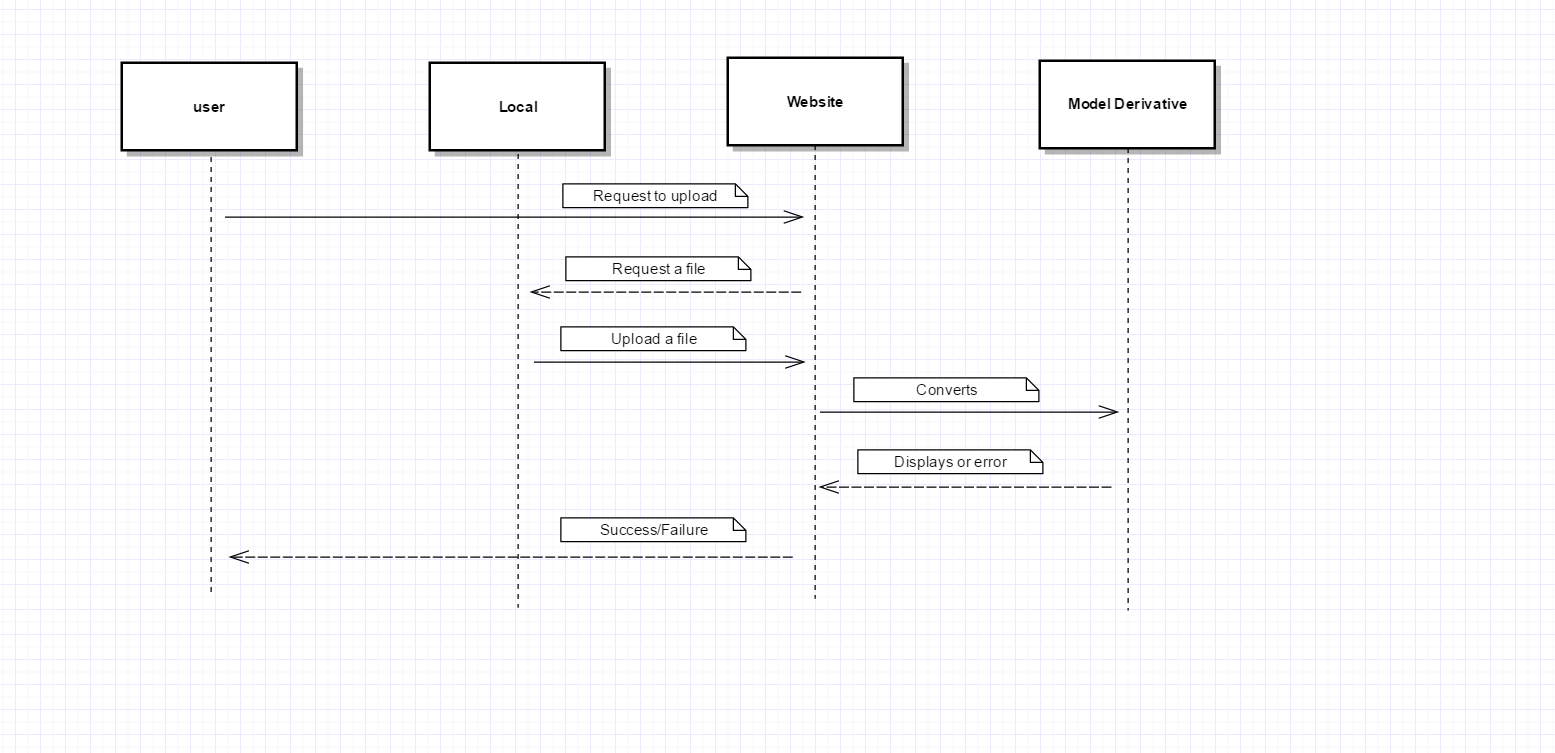
\includegraphics[scale=0.5]{localUpload.png}
	\caption{local file upload UML}
\end{figure}

\subsubsection{Design rationale}
	The reason for only letting users only use the CAD drawing file types because the files need to be converted to an SVF file to be used in the viewer. The conversion to SVF files is done using the model derivative api, and this api can only convert files that are CAD drawing files. 

\subsection{Non-local file upload}
	The user should be able to  access their files that are on an outside storage device and then upload these files to the website. There should be a button that the user can use to login to there outside storage. once logged in the user should be able to navigate to the file that they would like to use and then select that file to be uploaded. The website should verify that the selected file is of the correct file type and size. The website should also convert the file to an SVF file that the viewer can use. If for any reason there is a failure in the file upload then the user should be notified of that failure and informed of what to do.

\subsection{Interface viewpoint for non-local file upload}
\begin{itemize}
	\item[]\textbf{non-local upload button} This button should be easy for the user to identify in the main area of the web page. Once the user has pressed the button they should be prompted to login to the Autodesk account that they are trying to access.
	\item[]\textbf{user login} Using the data management api the user will be asked to login to there Autodesk account to receive an authentication token. Once logged in the user will have access to any of there Autodesk storage systems. 
	\item[]\textbf{file type verification} Once a file has been sent to the website from the outside storage should, it verify that the file is actually usable. This should be done by checking that if the file is a CAD drawing file type that can be converted into an SVF file that is used by the viewer. If the file is a usable file then the 	
	website should simply proceed and convert the file. If the file is not the correct file type then the user should be notified of this and prompted to select a different file.  
	\item[]\textbf{file selection} After the user has access they should then be able to navigate to the correct storage system their file is in and gain access to their files. Once a file is selected it should then be returned to the website. If returning the file is unsuccessful then the user should be notified and prompted to try 
	again.
	\item[]\textbf{file size verification} Large file may not work well in the viewer, in this case the website should determine if a file is to large for the viewer to handle. If the file the user has selected is to large then the user should be 		
	notified that the selected file is to large and be prompted to select a different file.
	\item[]\textbf{file conversion} The file conversion will be done through the use of the forge model derivative api. If the conversion request was successful then the file should be added to the current list of viewable models and also placed in the viewer described in section \ref{modelView}. If the conversion request is unsuccessful then the user should
	 be notified that their file could not be converted. 
\end{itemize}

\subsubsection{Design relationships}
	The user will gain access to there files through the use of the data management api described in section %add ref

	The uploaded file will be sent to the model derivative described in section \ref{model derivative} after the file type is verified.
	
	The converted file will be sent to the viewer described in section \ref{modelView}. 
  
\subsubsection{design constraints} 
	require that the file or file that the user is wanting to upload be located in the outside storage that they are wanting to use. They will also only be able use CAD drawing file when uploading a file to the website.  

\begin{figure}[ht]
	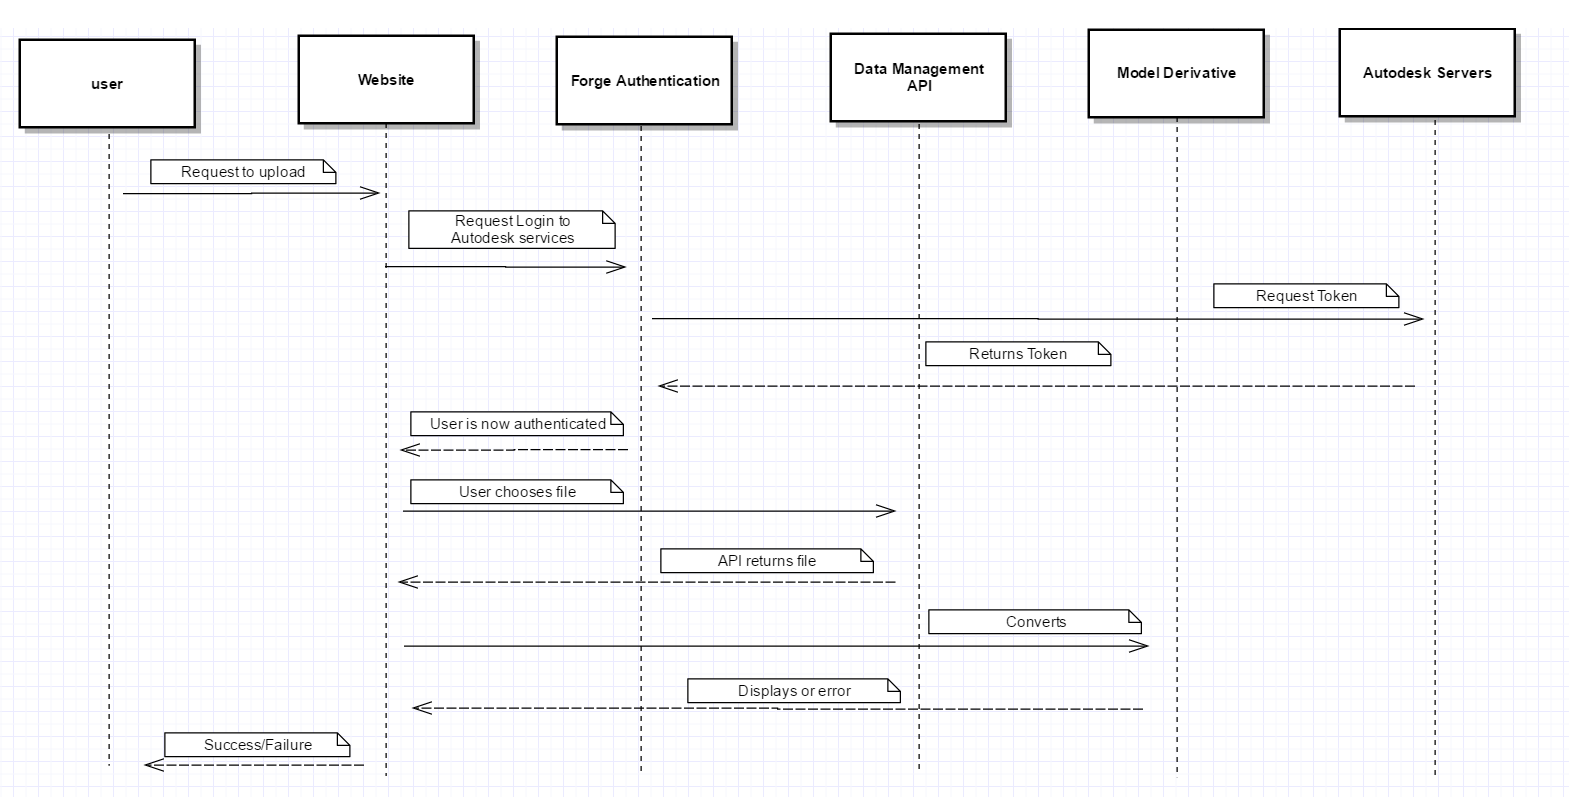
\includegraphics[scale=0.40]{nonLocalUpload.png}
	\caption{non-local file upload UML}
\end{figure}



\subsubsection{Design rationale}
	The reason for only letting users only use the CAD drawing file types because the files need to be converted to an SVF file to be used in the viewer. The conversion to SVF files is done using the model derivative api, and this api can only convert files that are CAD drawing files. 

\subsection{Mobile device connection}
	The user should be able to connect their mobile device to the websites current session through the use of a QR code on the web page. The user will need to have a some way to scan the QR code with their mobile device. 

\subsection{Mobile device connection Interface viewpoint}
\begin{description}
	\item[]\textbf{QR code} There should be a QR code generated at the beginning of every session on the web page. This will be done through the use of a jquery plug-in that generates QR codes. This plug-in can be found at \href{https://github.com/jeromeetienne/jquery-qrcode}{https://github.com/jeromeetienne/jquery-qrcode}. The QR code should be somewhere on the web page that is easy for the user to find. 
	\item[]\textbf{QR scanner} The user will need to have a way to scan the QR code. This will most likely be done through the use of an application on the users phone that will use there camera to scan the QR code. Any application that the user gets to scan the code should all work with the QR code on the website so there is no need to suggest a specific QR scanner to the user. 
	\item[]\textbf{device connection} Once the user has successfully scanned the QR code their device should notify them that they are being connected to the current session. If there is any reason that the device could not connect to the session then the user should be notified that the connection has failed and advise them to try to connect again.
	\item[]\textbf{device View} After the device has successfully connected to the current session then the user should see the exact same thing that is currently being displayed in the viewer. It should look as though there is two of the same images on the screen, this is for the use of viewing the object in a VR environment.  
\end{description}

\subsection{File conversion}
\label{model derivative} 
	The file conversion will be done using the forge model derivative api. This api will be sent a file anytime that one is uploaded to the website whether it be uploaded locally or uploaded from an outside storage device. The api should accept and CAD drawing files however, if a file is unable to be converted then the user should be notified. Once the api is done with the conversion then the it should send back the converted SVF file. 

\subsection{Interaction viewpoint for file conversion}
\begin{description}
	\item[]\textbf{conversion api} We will be using the forge model derivative api to convert the files uploaded to the website. We will be using this api because it is free and allows us to convert the files into the exact type of file used by the forge viewer api that we are also using. 
	\item[]\textbf{file conversions} Once a user has selected and uploaded the CAD drawing file that they would like to use it is then sent to the model derivative api. The api will take the file and then convert it from the current file format to an SVF file. After the file is converted it should be sent back to the website.
	\item[]\textbf{converted file} The converted file will be placed in the list of viewable models that can be selected as well as loaded into the viewer and should be seen by the user in the viewer.
	\item[]\textbf{conversion failure} If the file the user was trying to upload could not be converted by the api it will return a failed request. If a failed request is received then the user should be notified that their file fail to be convert. There is also the posibility that the translation has timed out. If this happens the user should be notified of the failure and then be prompted to try uploading the file again.
\end{description}

\begin{figure}[ht]
	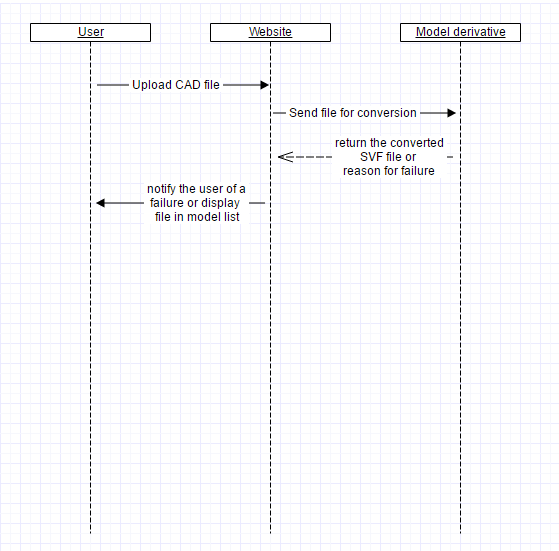
\includegraphics[scale=0.7]{conversionUML.png}
	\caption{File conversion interaction UML}
\end{figure}

\newpage
\subsection{Data Authentication}
\label{Two legged} 
	If there are resources a user can access without needing to provide permissions the 2 legged authentication system will address this. This takes use of the Forge's Data Authentication API and their OAuth rest points. The application will have a 32 character string that serves as the "client ID" and there will also be a client secret (which act as the password) both will given as a query parameter. 
\subsection{Interaction viewpoint for two legged authentication}
	Application requires resources from the Autodesk API and/or servers that do not need a users permissions. Application uses the POST authenticate endpoint to send client ID and secret along with any necessary scopes. Upon successful validation of credentials, access token is returned. When the token expires the process must be repeated.
\subsection{Design Concerns}
	The data must be secure and the exchange must be quick. A drawback of using Autodesk API and/or servers is the heavy reliance on it. The performance of the application is dependent on Autodesk, if the servers are slow or down, so is the application.
\subsection{Elements}
\begin{description}
	\item[]\textbf{Application} has a Client ID and Client Secret associated with it.
	\item[]\textbf{Client ID} acts as application username, 32 character string and passed as the client id query
	\item[]\textbf{Client secret} is the application password, 16 character string and passed as the client secret query
	\item[]\textbf{Access token} is returned at the end of a successful authentication flow, 28 character string used for subsequent API calls to the Forge platform. 
\end{description}

\begin{figure}[ht]
	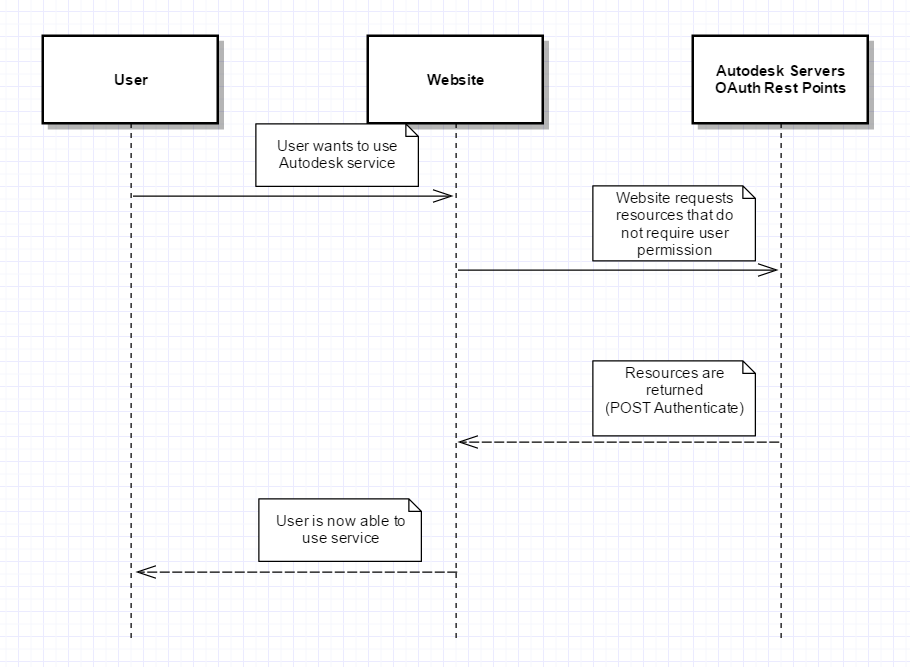
\includegraphics[scale=0.7]{Authentication2legged.png}
	\caption{Two legged OAuth UML sequence diagram}
\end{figure}

\subsection{Data Authentication}
\label{Three legged} 
	If there are resources the application requires that also require the permissions of the user. Then the 3 legged authentication will be used. This takes use of the Forge's Data Authentication API and their OAuth rest points. 
\subsection{Interaction viewpoint for two legged authentication}
	Application requires resources from the Autodesk API and/or servers that need a users permissions. Forge platform requires use of the "Authorization Code" grant type. User will be redirected to the Autodesk login (GET authorize endpoint). The user will have to register a new account if they do not have one. Then the user must explicitly accept the permissions the application requests. Using the callback URL the user is redirected to the application with a authorization code. With the code, client id and client secret, the application calls the POST gettoken endpoint. When successful the access token and refresh token are returned. The application is now able to obtain the resources needed. If the token expires the refresh token can use the POST refreshtoken endpoint to get a new access token. 
\subsection{Design Concerns}
	The data must be secure and the exchange must be quick. A drawback of using Autodesk API and/or servers is the heavy reliance on it. The performance of the application is dependent on Autodesk, if the servers are slow or down, so is the application. Three legged authentication also requires the login and permission of a user. If the user does not want or cannot provide permission then they are unable to use the application. Another concern is that the user must already own an account, if they do not they will have to create one. 
\subsection{Elements}
\begin{description}
	\item[]\textbf{Application} has a Client ID and Client Secret associated with it.
	\item[]\textbf{Client ID} acts as application username, 32 character string and passed as the client id query
	\item[]\textbf{Client secret} is the application password, 16 character string and passed as the client secret query
	\item[]\textbf{Access token} is returned at the end of a successful authentication flow, 28 character string used for subsequent API calls to the Forge platform. 
	\item[]\textbf{Callback URL} is the URL the user started from before they were redirected to the Autodesk login. It is necessary in order to bring the user back to the website.
	\item[]\textbf{Authorization code} is passed through the code query parameter when the user is returned to the application via the callback URL. Using POST gettoken endpoints as well as the client ID, client secret and this code, the application is able to receive an access token. The authorization code is 40 character string.
	\item[]\textbf{Refresh token} can use the POST refreshtoken endpoint to get new three-legged access tokens with having to have the user repeat logging in. Refresh tokens are 42 characters strings.

\end{description}

\begin{figure}[ht]
	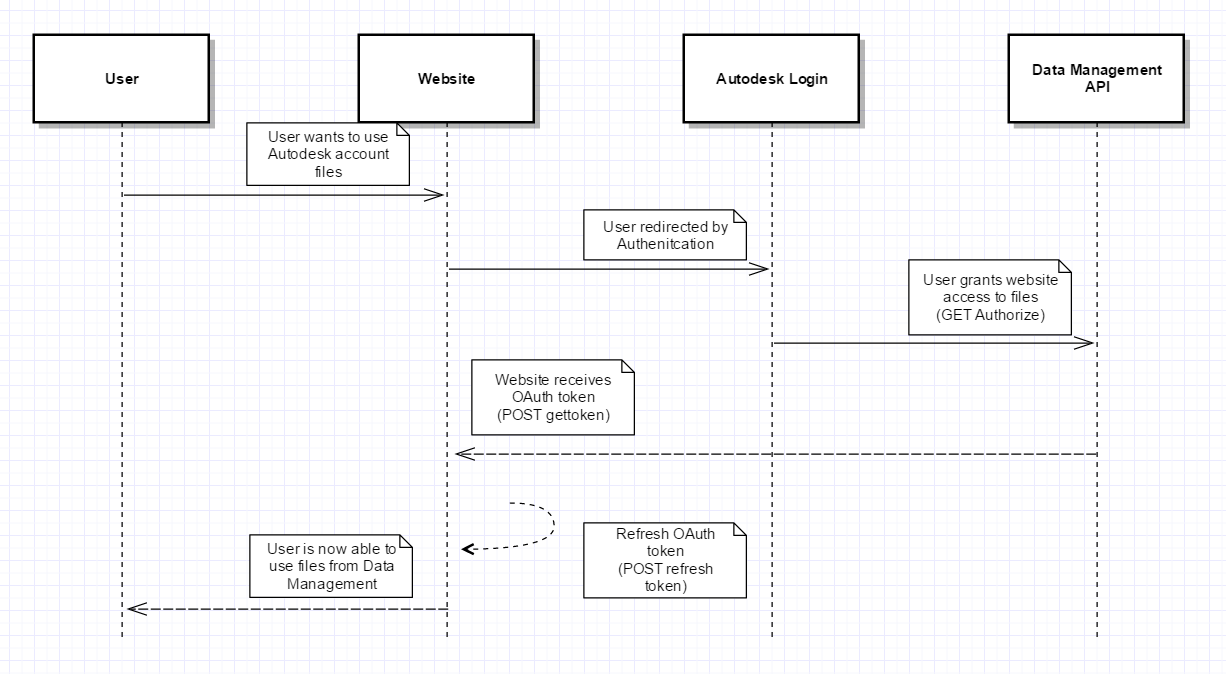
\includegraphics[scale=0.55]{Authentication3legged.png}
	\caption{Three legged OAuth UML sequence diagram}
\end{figure}

\subsection{Data Management API}
\label{A360} 
	A360 Personal requires 3-legged authorization for the application to access data. Then allows users to choose personal files for the application to use.
\subsection{Context viewpoint for Data Management API}
	
\subsection{Design Concerns}
	Since all data that comes from A360 belongs to an account, it is assumed that a user first off, is registered and has an account. Furthermore, that the user logins in and through the Data Authentication API provides the permissions to the application to allow the use of A360's resources. Second is that files actually exist in the accounts storage, if there are no files the user has nothing to choose to use. If the user does not choose a CAD file this issue is not caught at this stage in the application, it is done later.
\subsection{Elements}
\subsubsection{Entities}
\begin{description}
	\item[]\textbf{Users} 
	\item[]\textbf{Data Management API}
	\item[]\textbf{Data Authentication API}
\end{description}
\subsubsection{Relationships}
\begin{description}
	\item[]\textbf{User and Data Authentication's Relationship}: The user must login their Autodesk account and then provide explicit permissions for resources. This will give the authentication the okay to begin sending tokens.
	\item[]\textbf{User and Data Managements's Relationship}: The user will select the files they want from the data management and the data management API will provide those files to the user.
	\item[]\textbf{Data Authentication and Data Managements's Relationship}: The data authentication API will keep the token that allows the data management API to send resources to the application.
\end{description}
\subsubsection{Constraints}
\begin{description}
	\item[]\textbf{Users} must have a Autodesk account registered as well as files within the data management API.

\end{description}

\begin{figure}[ht]
	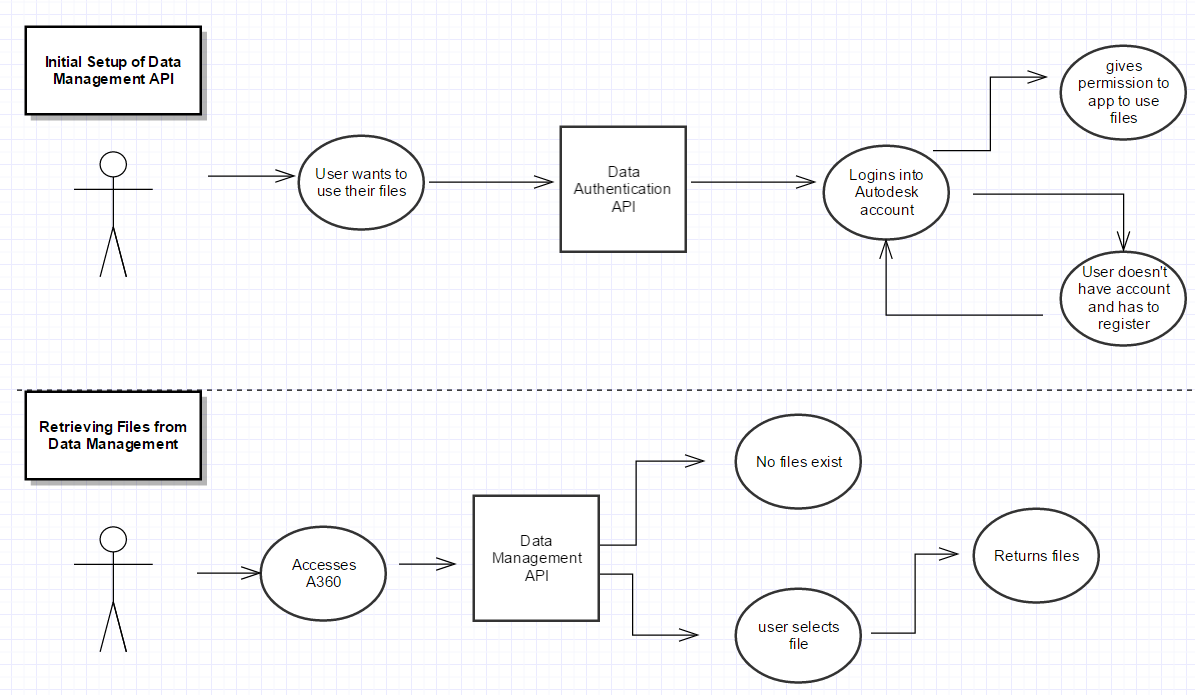
\includegraphics[scale=0.6]{DataManageUseCase.png}
	\caption{Data Management UML use case diagram}
\end{figure}

\end{document}

%@misc{a javascript library for building user interfaces - react,
 %title={A JavaScript library for building user interfaces - React},
 %url={https://facebook.github.io/react/},
 %journal={A JavaScript library for building user interfaces - React}, 
 %publisher={Facebook.com}}

